\documentclass[12pt,a4paper]{article}

% ─── Page Layout ───────────────────────────────────────────────────────────────
\usepackage[a4paper, margin=0.8in, headheight=14pt]{geometry}

% ─── Fonts (XeLaTeX) ───────────────────────────────────────────────────────────
\usepackage{fontspec}
\usepackage{unicode-math}
\setmainfont{TeX Gyre Pagella}
\setmonofont[Scale=0.88]{TeX Gyre Cursor}
\setmathfont{Latin Modern Math}

% ─── Packages ──────────────────────────────────────────────────────────────────
\usepackage{xcolor}
\usepackage{colortbl}
\usepackage{titlesec}
\usepackage{enumitem}
\usepackage{tabularx}
\usepackage{booktabs}
\usepackage{array}
\usepackage{amsmath}
\usepackage{tikz}
\usetikzlibrary{shapes.geometric, arrows.meta, positioning, calc, fit, decorations.pathreplacing, patterns}
\usepackage{tcolorbox}
\tcbuselibrary{skins, breakable}
\usepackage{hyperref}
\usepackage{fancyhdr}
\usepackage{graphicx}
\usepackage{microtype}
\hyphenpenalty=10000
\exhyphenpenalty=10000
\sloppy
\usepackage{caption}
\usepackage{setspace}
\usepackage{multirow}
\usepackage{tocloft}

% ─── Q&A helper ────────────────────────────────────────────────────────────────
\newcommand{\Q}[1]{\textbf{#1}\par\noindent\ignorespaces}

% ─── Colour Palette ────────────────────────────────────────────────────────────
\definecolor{myred}{RGB}{196,30,58}
\definecolor{mydark}{RGB}{30,30,50}
\definecolor{mygreen}{RGB}{14,120,80}
\definecolor{myteal}{RGB}{0,130,140}
\definecolor{myamber}{RGB}{180,100,0}
\definecolor{mypurple}{RGB}{100,30,160}
\definecolor{mygray}{RGB}{246,247,249}
\definecolor{mgframe}{RGB}{180,185,200}
\definecolor{watermark}{RGB}{145,150,170}
\definecolor{hdrred}{RGB}{250,232,235}
\definecolor{hdrgreen}{RGB}{220,244,233}
\definecolor{hdrteal}{RGB}{220,242,244}
\definecolor{hdramber}{RGB}{253,242,215}
\definecolor{hdrpurple}{RGB}{238,228,255}
\definecolor{hdrgray}{RGB}{238,240,245}
\definecolor{rowalt}{RGB}{250,251,253}

% ─── Section Formatting ────────────────────────────────────────────────────────
\titleformat{\section}
  {\large\bfseries\color{myred}}{\thesection.}{0.5em}{}
  [\vspace{1pt}{\color{myred}\rule{\linewidth}{0.8pt}}]
\titleformat{\subsection}
  {\normalsize\bfseries\color{myteal}}{\thesubsection}{0.5em}{}
\titlespacing*{\section}{0pt}{18pt}{7pt}
\titlespacing*{\subsection}{0pt}{11pt}{4pt}

% ─── Paragraph ─────────────────────────────────────────────────────────────────
\setlength{\parindent}{0pt}
\setlength{\parskip}{4pt}

% ─── TOC Styling ───────────────────────────────────────────────────────────────
\renewcommand{\cfttoctitlefont}{\large\bfseries\color{myred}}
\renewcommand{\cftaftertoctitle}{\par\noindent{\color{myred}\rule{\linewidth}{0.8pt}}}
\setlength{\cftbeforetoctitleskip}{0pt}
\setlength{\cftaftertoctitleskip}{6pt}
\renewcommand{\cftsecfont}{\normalsize\bfseries\color{mydark}}
\renewcommand{\cftsecpagefont}{\normalsize\bfseries\color{mydark}}
\renewcommand{\cftsecleader}{\cftdotfill{\cftdotsep}}
\setlength{\cftbeforesecskip}{7pt}
\renewcommand{\cftsubsecfont}{\small\color{mydark}}
\renewcommand{\cftsubsecpagefont}{\small\color{mydark}}
\setlength{\cftbeforesubsecskip}{3pt}
\setlength{\cftsubsecindent}{1.4em}

% ─── Table helpers ─────────────────────────────────────────────────────────────
\renewcommand{\arraystretch}{1.45}
\setlength{\tabcolsep}{6pt}
\arrayrulecolor{mydark}
\newcolumntype{B}[1]{>{\small\bfseries\raggedright\arraybackslash}m{#1}}
\newcolumntype{Y}{>{\small\raggedright\arraybackslash}X}
\renewcommand{\tabularxcolumn}[1]{m{#1}}

% ─── Header / Footer ───────────────────────────────────────────────────────────
\pagestyle{fancy}
\fancyhf{}
\fancyhead[L]{\small\color{myred}\textbf{EC304}\;\color{mydark}--- Network Theory}
\fancyhead[R]{\small\color{myteal}\textbf{Module 3 Notes}}
\fancyfoot[C]{\small\color{mydark}\thepage}
\fancyfoot[R]{\small\color{watermark}\textit{\copyright\ Biraj}}
\renewcommand{\headrulewidth}{0.5pt}
\renewcommand{\footrulewidth}{0.3pt}

% ─── Hyperref ──────────────────────────────────────────────────────────────────
\hypersetup{
  colorlinks=true, linkcolor=myteal, urlcolor=myteal,
  pdfauthor={Biraj Sarkar (CGEC)},
  pdftitle={EC304 --- Module 3 Notes: Laplace Transforms, Network Transients and Initial Conditions}
}

% ─── tcolorbox styles ──────────────────────────────────────────────────────────
\tcbset{
  tikzbox/.style={
    colback=mygray, colframe=mgframe, boxrule=0.6pt, arc=4pt,
    left=8pt, right=8pt, top=6pt, bottom=6pt,
    colbacktitle=mgframe, coltitle=mydark,
    fonttitle=\small\bfseries
  },
  defbox/.style={
    colback=hdrgreen, colframe=mygreen, boxrule=0.8pt, arc=4pt,
    left=9pt, right=9pt, top=6pt, bottom=6pt,
    colbacktitle=mygreen, coltitle=white,
    fonttitle=\small\bfseries
  },
  formulabox/.style={
    colback=hdrteal, colframe=myteal, boxrule=0.8pt, arc=4pt,
    left=9pt, right=9pt, top=7pt, bottom=7pt,
    colbacktitle=myteal, coltitle=white,
    fonttitle=\small\bfseries
  },
  examplebox/.style={
    colback=hdramber, colframe=myamber, boxrule=0.8pt, arc=4pt,
    left=9pt, right=9pt, top=6pt, bottom=6pt,
    colbacktitle=myamber, coltitle=white,
    fonttitle=\small\bfseries
  },
  masonbox/.style={
    colback=hdrpurple, colframe=mypurple, boxrule=0.8pt, arc=4pt,
    left=9pt, right=9pt, top=6pt, bottom=6pt,
    colbacktitle=mypurple, coltitle=white,
    fonttitle=\small\bfseries
  },
  exambox/.style={
    colback=hdrpurple, colframe=mypurple, boxrule=1pt, arc=5pt,
    left=10pt, right=10pt, top=8pt, bottom=8pt,
    colbacktitle=mypurple, coltitle=white,
    fonttitle=\bfseries,
    breakable, title after break={\textbf{Frequently Asked / Viva Questions (contd.)}}
  }
}
\tcbset{breakable}
\tcbset{after={\color{black}}}

% ─── TikZ styles ───────────────────────────────────────────────────────────────
\tikzset{
  circnode/.style={circle, draw=myteal, fill=hdrteal, inner sep=2pt, minimum size=6pt},
  sourcenode/.style={circle, draw=myred, fill=hdrred, minimum size=0.9cm, font=\small\bfseries, align=center},
  depnode/.style={diamond, draw=myred, fill=hdrred, minimum size=1.0cm, font=\small\bfseries, align=center},
  block/.style={rectangle, draw=myteal, fill=hdrteal, text width=2.4cm, align=center, minimum height=0.95cm, font=\small, rounded corners=3pt, line width=0.7pt},
  arrow/.style={-Stealth, thick, color=mydark},
  redarrow/.style={-Stealth, thick, color=myred},
  line/.style={thick, color=mydark}
}

\begin{document}

% ─── Title Block ───────────────────────────────────────────────────────────────
\begin{center}
  {\LARGE\bfseries\color{myred} EC304 --- Network Theory}\\[5pt]
  {\normalsize\color{mydark} Semester III \quad$\bullet$\quad 3L:0T:0P \quad$\bullet$\quad 3 Credits}\\[3pt]
  {\normalsize\color{myteal}\textbf{Module 3 Exam Notes: Laplace Transforms, Network Transients \& Initial Conditions}}\\[3pt]
  {\small\color{mydark} CGEC \;$|$\; B.Tech ECE (2023--27) \;$|$\; \textit{Biraj Sarkar}}
\end{center}
\vspace{2pt}\noindent{\color{myred}\rule{\linewidth}{1.5pt}}\vspace{2pt}

\hypersetup{linkcolor=mydark}
\tableofcontents
\hypersetup{linkcolor=myteal}
\newpage

% ===============================================================================
% SECTION 1: SINGULARITY FUNCTIONS AND WAVEFORM SYNTHESIS
% ===============================================================================
\section{Singularity Functions and Waveform Synthesis}

Singularity functions (also referred to as switching functions or test signals) are a family of mathematical idealizations exhibiting discontinuities or discontinuous derivatives. In linear circuit theory, they model switching actions, sharp current/voltage pulses, and sudden transients.

\subsection{Standard Singularity Functions}

\begin{tcolorbox}[defbox, title={\textbf{Definitions of Core Singularity Functions}}]
\begin{enumerate}[leftmargin=*, itemsep=4pt]
  \item \textbf{Unit Step Function $u(t)$:} Models the instantaneous closing or opening of an ideal switch at $t = 0$:
  \begin{equation}
    u(t) = \begin{cases} 0, & t < 0 \\ 1, & t > 0 \end{cases} \qquad \text{Delayed: } u(t - t_0) = \begin{cases} 0, & t < t_0 \\ 1, & t > t_0 \end{cases}
  \end{equation}
  \item \textbf{Unit Impulse (Dirac Delta) Function $\delta(t)$:} Defined as the distributional derivative of the unit step function:
  \begin{equation}
    \delta(t) = \frac{du(t)}{dt}, \quad \delta(t) = 0 \text{ for } t \ne 0, \quad \int_{-\infty}^{\infty} \delta(t)\,dt = 1
  \end{equation}
  \textbf{Sifting (Sampling) Property:}
  \begin{equation}
    \int_{-\infty}^{\infty} f(t)\,\delta(t - t_0)\,dt = f(t_0)
  \end{equation}
  \item \textbf{Unit Ramp Function $r(t)$:} Represents a linearly growing excitation starting at $t=0$:
  \begin{equation}
    r(t) = \int_{-\infty}^t u(\tau)\,d\tau = t\,u(t) = \begin{cases} 0, & t < 0 \\ t, & t \ge 0 \end{cases}
  \end{equation}
  \item \textbf{Unit Doublet $\delta'(t)$:} The time derivative of the unit impulse function:
  \begin{equation}
    \delta'(t) = \frac{d\delta(t)}{dt}, \qquad \int_{-\infty}^\infty f(t)\,\delta'(t - t_0)\,dt = -f'(t_0)
  \end{equation}
\end{enumerate}
\end{tcolorbox}

\begin{tcolorbox}[formulabox, title={\textbf{Hierarchy of Singularity Functions}}]
The standard singularity functions form a continuous calculus chain linked by differentiation and integration:
\begin{equation}
  \cdots \xleftarrow{\frac{d}{dt}} \delta'(t) \xleftarrow{\frac{d}{dt}} \delta(t) \xleftarrow{\frac{d}{dt}} u(t) \xleftarrow{\frac{d}{dt}} r(t) \xleftarrow{\frac{d}{dt}} \frac{t^2}{2}u(t) \cdots
\end{equation}
\end{tcolorbox}

\subsection{Waveform Synthesis Technique}

Any arbitrary piecewise-linear or stepped signal can be synthesized systematically as a linear algebraic sum of delayed ramp functions and delayed step functions:
\begin{equation}
  v(t) = \sum_{k=0}^{N} \Delta m_k\, r(t - t_k) + \sum_{j=0}^{M} \Delta v_j\, u(t - t_j)
\end{equation}
where $\Delta m_k = m_k - m_{k-1}$ is the change in slope at breakpoint $t_k$, and $\Delta v_j$ is the abrupt jump in amplitude at breakpoint $t_j$.

\begin{tcolorbox}[tikzbox, title={\textbf{TikZ Schematic: Synthesis of a Trapezoidal Pulse from Singularity Functions}}]
\begin{center}
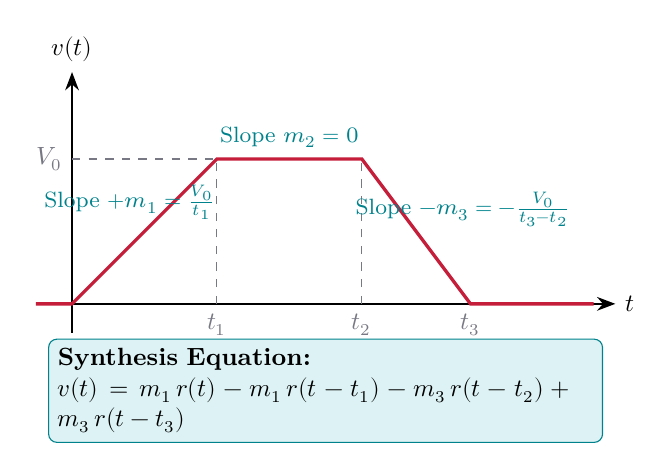
\begin{tikzpicture}[scale=0.92, every node/.style={font=\small}]
  % Axes
  \draw[-Stealth, thick] (-0.5,0) -- (7.5,0) node[right] {$t$};
  \draw[-Stealth, thick] (0,-0.4) -- (0,3.2) node[above] {$v(t)$};

  % Trapezoid waveform
  \draw[very thick, color=myred] (-0.5,0) -- (0,0) -- (2,2) -- (4,2) -- (5.5,0) -- (7.2,0);

  % Dashed projection lines
  \draw[dashed, color=mydark!60] (2,0) node[below] {$t_1$} -- (2,2);
  \draw[dashed, color=mydark!60] (4,0) node[below] {$t_2$} -- (4,2);
  \draw[dashed, color=mydark!60] (5.5,0) node[below] {$t_3$} -- (5.5,0);
  \draw[dashed, color=mydark!60] (0,2) node[left] {$V_0$} -- (2,2);

  % Annotations
  \node[color=myteal, font=\footnotesize] at (0.8, 1.4) {Slope $+m_1 = \frac{V_0}{t_1}$};
  \node[color=myteal, font=\footnotesize] at (3.0, 2.3) {Slope $m_2 = 0$};
  \node[color=myteal, font=\footnotesize] at (5.4, 1.3) {Slope $-m_3 = -\frac{V_0}{t_3 - t_2}$};

  % Equation Box
  \node[draw=myteal, fill=hdrteal, rounded corners=3pt, text width=6.8cm, align=left] at (3.5, -1.2) {
    \textbf{Synthesis Equation:}\\
    $v(t) = m_1\,r(t) - m_1\,r(t-t_1) - m_3\,r(t-t_2) + m_3\,r(t-t_3)$
  };
\end{tikzpicture}
\end{center}
\end{tcolorbox}

\begin{tcolorbox}[examplebox, title={\textbf{Step-by-Step Example: Waveform Synthesis and its Transform}}]
\textbf{Problem:} Express a triangular pulse that rises linearly from $0$ to $10\text{ V}$ between $t=0$ and $t=2\text{ s}$, and drops instantaneously to zero at $t=2\text{ s}$. Determine its Laplace transform.

\textbf{Solution:}
\begin{enumerate}[leftmargin=*]
  \item Between $t=0$ and $t=2$, the waveform has a constant slope $m_1 = \frac{10 - 0}{2 - 0} = +5\text{ V/s}$. It starts at $t=0$, represented as $5\,r(t)$.
  \item At $t=2\text{ s}$, the ramp must be cancelled by subtracting an identical ramp of slope $5$: $-5\,r(t-2)$.
  \item At $t=2\text{ s}$, the voltage must also jump downwards instantaneously by $-10\text{ V}$ to reach $0$: $-10\,u(t-2)$.
  \item Synthesized time-domain expression:
  \begin{equation}
    v(t) = 5\,r(t) - 5\,r(t-2) - 10\,u(t-2)
  \end{equation}
  \item Applying the time-shifting property of the Laplace transform:
  \begin{equation}
    V(s) = \frac{5}{s^2} - \frac{5}{s^2}\,e^{-2s} - \frac{10}{s}\,e^{-2s} = \frac{5}{s^2}\left[1 - e^{-2s}(1 + 2s)\right]
  \end{equation}
\end{enumerate}
\end{tcolorbox}

% ===============================================================================
% SECTION 2: THE LAPLACE TRANSFORM AND PROPERTIES
% ===============================================================================
\section{The Laplace Transform and Operational Theorems}

The unilateral (one-sided) Laplace transform is an essential mathematical tool for solving linear, time-invariant (LTI) differential equations with non-zero initial boundary conditions.

\subsection{Definition and Region of Convergence}

\begin{tcolorbox}[defbox, title={\textbf{Unilateral Laplace Transform}}]
Let $f(t)$ be a continuous or piecewise-continuous function defined for $t \ge 0$. The unilateral Laplace transform $\mathcal{L}\{f(t)\} = F(s)$ is:
\begin{equation}
  F(s) = \int_{0^-}^\infty f(t)\,e^{-st}\,dt
\end{equation}
where $s = \sigma + j\omega$ is the complex frequency variable. The lower integration limit $0^- \equiv \lim_{\epsilon \to 0^+} (0 - \epsilon)$ ensures that singularity functions (such as $\delta(t)$) acting at $t=0$ are rigorously integrated and accounted for.
\end{tcolorbox}

\subsection{Operational Theorems for Circuit Analysis}

\par\vspace{6pt}\noindent
\begingroup
\setlength{\tabcolsep}{5pt}
\setlength{\extrarowheight}{3pt}
\renewcommand{\arraystretch}{1.38}
\begin{tabularx}{\linewidth}{|B{3.4cm}|B{3.2cm}|Y|}
\hline
\multicolumn{1}{|c|}{\textbf{Property / Theorem}} & \multicolumn{1}{c|}{\textbf{Time Domain $f(t)$}} & \multicolumn{1}{c|}{\textbf{Frequency Domain $F(s)$}} \\
\hline
Linearity & $a_1 f_1(t) + a_2 f_2(t)$ & $a_1 F_1(s) + a_2 F_2(s)$ \\
\hline
First Shifting (Frequency) & $e^{-at} f(t)$ & $F(s + a)$ \\
\hline
Second Shifting (Time) & $f(t - t_0)\,u(t - t_0)$ & $e^{-s t_0} F(s) \quad (t_0 \ge 0)$ \\
\hline
Time Differentiation (1st) & $\dfrac{df(t)}{dt}$ & $s F(s) - f(0^-)$ \\
\hline
Time Differentiation (2nd) & $\dfrac{d^2f(t)}{dt^2}$ & $s^2 F(s) - s f(0^-) - f'(0^-)$ \\
\hline
Time Integration & $\displaystyle\int_{0^-}^t f(\tau)\,d\tau$ & $\dfrac{F(s)}{s}$ \\
\hline
Frequency Differentiation & $t\,f(t)$ & $-\dfrac{d}{ds}F(s)$ \\
\hline
Time Convolution & $f_1(t) * f_2(t)$ & $F_1(s) \cdot F_2(s)$ \\
\hline
Initial Value Theorem & $\displaystyle\lim_{t \to 0^+} f(t)$ & $\displaystyle\lim_{s \to \infty} s F(s)$ \quad (if limit exists) \\
\hline
Final Value Theorem & $\displaystyle\lim_{t \to \infty} f(t)$ & $\displaystyle\lim_{s \to 0} s F(s)$ \quad (poles of $sF(s)$ in LHP) \\
\hline
Periodic Function ($T$) & $f(t) = f(t + T)$ & $\dfrac{1}{1 - e^{-sT}} \displaystyle\int_0^T f(t) e^{-st}\,dt$ \\
\hline
\end{tabularx}
\endgroup
\vspace{12pt}

\begin{tcolorbox}[masonbox, title={\textbf{Critical Examination Note: Validity of the Final Value Theorem (FVT)}}]
The Final Value Theorem $\lim_{t \to \infty} f(t) = \lim_{s \to 0} s F(s)$ is valid \textbf{if and only if} the function $f(t)$ possesses a finite, stable steady-state limit as $t \to \infty$. Mathematically, this requires that all poles of $s F(s)$ reside strictly in the open left-half of the $s$-plane ($\text{Re}(s) < 0$).
\begin{itemize}[leftmargin=*]
  \item For $f(t) = \sin(\omega_0 t)$, $F(s) = \frac{\omega_0}{s^2 + \omega_0^2}$. Here $sF(s) = \frac{s\omega_0}{s^2 + \omega_0^2}$. Evaluating $\lim_{s \to 0} sF(s) = 0$, but $\lim_{t \to \infty}\sin(\omega_0 t)$ does not exist (it oscillates indefinitely). FVT fails because poles are on the $j\omega$-axis!
\end{itemize}
\end{tcolorbox}

\subsection{Standard Laplace Transform Pairs}

\par\vspace{6pt}\noindent
\begingroup
\setlength{\tabcolsep}{5pt}
\setlength{\extrarowheight}{2.5pt}
\renewcommand{\arraystretch}{1.35}
\begin{tabularx}{\linewidth}{|B{3.2cm}|B{3.0cm}|B{3.2cm}|Y|}
\hline
\multicolumn{1}{|c|}{\textbf{Signal $f(t)$}} & \multicolumn{1}{c|}{\textbf{$F(s)$}} & \multicolumn{1}{c|}{\textbf{Signal $f(t)$}} & \multicolumn{1}{c|}{\textbf{$F(s)$}} \\
\hline
$\delta(t)$ & $1$ & $u(t)$ & $\dfrac{1}{s}$ \\
\hline
$t\,u(t)$ & $\dfrac{1}{s^2}$ & $t^n\,u(t)$ & $\dfrac{n!}{s^{n+1}}$ \\
\hline
$e^{-at}\,u(t)$ & $\dfrac{1}{s + a}$ & $t\,e^{-at}\,u(t)$ & $\dfrac{1}{(s + a)^2}$ \\
\hline
$\sin(\omega t)\,u(t)$ & $\dfrac{\omega}{s^2 + \omega^2}$ & $\cos(\omega t)\,u(t)$ & $\dfrac{s}{s^2 + \omega^2}$ \\
\hline
$e^{-at}\sin(\omega t)\,u(t)$ & $\dfrac{\omega}{(s + a)^2 + \omega^2}$ & $e^{-at}\cos(\omega t)\,u(t)$ & $\dfrac{s + a}{(s + a)^2 + \omega^2}$ \\
\hline
\end{tabularx}
\endgroup
\vspace{12pt}

% ===============================================================================
% SECTION 3: INVERSE LAPLACE TRANSFORM AND PARTIAL FRACTIONS
% ===============================================================================
\section{Inverse Laplace Transform and Partial Fraction Expansion}

In network transient problems, the $s$-domain response is generally obtained as a rational transfer function $F(s) = \frac{P(s)}{Q(s)}$, where $P(s)$ and $Q(s)$ are polynomials in $s$ with real coefficients, and $\text{deg}(P) < \text{deg}(Q)$ (strictly proper).

\subsection{Decomposition Methodologies}

\begin{tcolorbox}[defbox, title={\textbf{Three Cases of Partial Fraction Expansion}}]
\begin{enumerate}[leftmargin=*, itemsep=4pt]
  \item \textbf{Case I: Distinct Real Roots (Simple Poles)}
  \begin{equation}
    F(s) = \frac{P(s)}{(s - p_1)(s - p_2)\cdots(s - p_n)} = \sum_{k=1}^n \frac{A_k}{s - p_k}
  \end{equation}
  The residues $A_k$ are evaluated by Heaviside's cover-up rule:
  \begin{equation}
    A_k = \lim_{s \to p_k} (s - p_k)\,F(s) \implies f(t) = \sum_{k=1}^n A_k\,e^{p_k t}\,u(t)
  \end{equation}

  \item \textbf{Case II: Repeated Real Roots (Multiple Poles of Order $m$)}
  \begin{equation}
    F(s) = \frac{P(s)}{(s - p)^m\,Q_1(s)} = \frac{B_m}{(s - p)^m} + \frac{B_{m-1}}{(s - p)^{m-1}} + \cdots + \frac{B_1}{s - p} + \cdots
  \end{equation}
  where the coefficients are given by:
  \begin{equation}
    B_{m-k} = \frac{1}{k!}\lim_{s \to p} \frac{d^k}{ds^k} \left[(s - p)^m\,F(s)\right], \quad k = 0, 1, \dots, m-1
  \end{equation}

  \item \textbf{Case III: Complex Conjugate Poles ($s = -\alpha \pm j\beta$)}
  \begin{equation}
    F(s) = \frac{C s + D}{(s + \alpha)^2 + \beta^2} = \frac{C(s + \alpha) + (D - C\alpha)}{(s + \alpha)^2 + \beta^2}
  \end{equation}
  The inverse transform yields a damped sinusoid:
  \begin{equation}
    f(t) = C e^{-\alpha t}\cos(\beta t) + \frac{D - C\alpha}{\beta} e^{-\alpha t}\sin(\beta t) = M e^{-\alpha t}\cos(\beta t - \theta)
  \end{equation}
  where $M = \sqrt{C^2 + \left(\frac{D - C\alpha}{\beta}\right)^2}$ and $\theta = \tan^{-1}\left(\frac{D - C\alpha}{\beta C}\right)$.
\end{enumerate}
\end{tcolorbox}

% ===============================================================================
% SECTION 4: EVALUATION OF INITIAL CONDITIONS
% ===============================================================================
\section{Evaluation of Initial Conditions in Electrical Networks}

Evaluating initial conditions at the switching instant ($t = 0^-$ and $t = 0^+$) is an absolute prerequisite for setting up transient differential equations and their Laplace counterparts.

\subsection{Physical Boundary and Continuity Principles}

\begin{tcolorbox}[defbox, title={\textbf{Energy Continuity Postulates}}]
\begin{enumerate}[leftmargin=*]
  \item \textbf{Conservation of Inductor Flux Linkage:} An inductor stores magnetic energy $W_m = \frac{1}{2} L i_L^2$. An instantaneous discontinuity in $i_L(t)$ requires infinite voltage ($v_L = L \frac{di}{dt} \to \infty$) and infinite instantaneous power, which is physically impossible in passive circuits without impulse voltage sources. Therefore:
  \begin{equation}
    i_L(0^+) = i_L(0^-)
  \end{equation}
  \item \textbf{Conservation of Capacitor Electric Charge:} A capacitor stores electrostatic energy $W_e = \frac{1}{2} C v_C^2$. An instantaneous discontinuity in $v_C(t)$ requires infinite current ($i_C = C \frac{dv_C}{dt} \to \infty$), which is physically impossible in passive circuits without impulse current sources. Therefore:
  \begin{equation}
    v_C(0^+) = v_C(0^-)
  \end{equation}
\end{enumerate}
\end{tcolorbox}

\subsection{Equivalent Circuits at $t=0^-$ and $t=0^+$}

\par\vspace{6pt}\noindent
\begingroup
\setlength{\tabcolsep}{5pt}
\setlength{\extrarowheight}{3pt}
\renewcommand{\arraystretch}{1.38}
\begin{tabularx}{\linewidth}{|B{2.2cm}|B{3.2cm}|B{3.2cm}|Y|}
\hline
\multicolumn{1}{|c|}{\textbf{Element}} & \multicolumn{1}{c|}{\textbf{DC Steady State ($t = 0^-$)}} & \multicolumn{1}{c|}{\textbf{At $t = 0^+$ (with initial state)}} & \multicolumn{1}{c|}{\textbf{At $t = 0^+$ (zero initial state)}} \\
\hline
Resistor ($R$) & Resistor $R$ ($v_R = i_R R$) & Resistor $R$ ($v_R = i_R R$) & Resistor $R$ ($v_R = i_R R$) \\
\hline
Inductor ($L$) & Short Circuit ($v_L = 0$) & Current Source $I_0 = i_L(0^-)$ & Open Circuit ($i_L(0^+) = 0$) \\
\hline
Capacitor ($C$) & Open Circuit ($i_C = 0$) & Voltage Source $V_0 = v_C(0^-)$ & Short Circuit ($v_C(0^+) = 0$) \\
\hline
\end{tabularx}
\endgroup
\vspace{12pt}

\subsection{Evaluation of Higher Derivatives at $t = 0^+$}

To evaluate higher-order derivatives such as $\frac{di}{dt}(0^+)$, $\frac{dv_C}{dt}(0^+)$, and $\frac{d^2i}{dt^2}(0^+)$:
\begin{enumerate}[leftmargin=*]
  \item Write the loop KVL and nodal KCL equations for $t > 0$ containing derivative terms:
  \begin{equation}
    v_L(t) = L\,\frac{di_L(t)}{dt} \implies \left.\frac{di_L}{dt}\right|_{t=0^+} = \frac{v_L(0^+)}{L}
  \end{equation}
  \begin{equation}
    i_C(t) = C\,\frac{dv_C(t)}{dt} \implies \left.\frac{dv_C}{dt}\right|_{t=0^+} = \frac{i_C(0^+)}{C}
  \end{equation}
  \item Calculate $v_L(0^+)$ and $i_C(0^+)$ directly by evaluating the network loop/node equations at the instant $t = 0^+$ using the known boundary values $i_L(0^+)$ and $v_C(0^+)$.
  \item Differentiate the general differential equation with respect to $t$, and evaluate the resulting relation at $t = 0^+$ to find the second derivative $\frac{d^2i}{dt^2}(0^+)$.
\end{enumerate}

\begin{tcolorbox}[examplebox, title={\textbf{Worked Example: Complete Evaluation of Initial Boundary Derivatives}}]
\textbf{Problem:} In a series RLC circuit ($R=10\,\Omega, L=1\text{ H}, C=0.1\text{ F}$), a DC voltage $V = 100\text{ V}$ is suddenly applied at $t=0$ by closing a switch. The circuit had no initial energy ($i_L(0^-)=0, v_C(0^-)=0$). Find $i(0^+)$, $\frac{di}{dt}(0^+)$, and $\frac{d^2i}{dt^2}(0^+)$.

\textbf{Solution:}
\begin{enumerate}[leftmargin=*]
  \item \textbf{At $t = 0^+$:}
  Due to continuity of inductor current, $i(0^+) = i_L(0^-) = 0\text{ A}$.
  Due to continuity of capacitor voltage, $v_C(0^+) = v_C(0^-) = 0\text{ V}$.
  \item \textbf{First derivative $\frac{di}{dt}(0^+)$:}
  Applying KVL around the loop for $t \ge 0$:
  \begin{equation}
    R\,i(t) + L\,\frac{di(t)}{dt} + v_C(t) = V
  \end{equation}
  Evaluating this at $t = 0^+$:
  \begin{equation}
    R\,i(0^+) + L\left.\frac{di}{dt}\right|_{t=0^+} + v_C(0^+) = V \implies 10(0) + 1 \cdot \left.\frac{di}{dt}\right|_{t=0^+} + 0 = 100
  \end{equation}
  \begin{equation}
    \left.\frac{di}{dt}\right|_{t=0^+} = \frac{100 - 0 - 0}{1} = 100\text{ A/s}
  \end{equation}
  \item \textbf{Second derivative $\frac{d^2i}{dt^2}(0^+)$:}
  Differentiating the KVL equation with respect to time $t$:
  \begin{equation}
    R\,\frac{di(t)}{dt} + L\,\frac{d^2i(t)}{dt^2} + \frac{dv_C(t)}{dt} = 0 \implies R\,\frac{di}{dt} + L\,\frac{d^2i}{dt^2} + \frac{i(t)}{C} = 0
  \end{equation}
  Evaluating at $t = 0^+$:
  \begin{equation}
    10(100) + 1 \cdot \left.\frac{d^2i}{dt^2}\right|_{t=0^+} + \frac{0}{0.1} = 0 \implies \left.\frac{d^2i}{dt^2}\right|_{t=0^+} = -1000\text{ A/s}^2
  \end{equation}
\end{enumerate}
\end{tcolorbox}

% ===============================================================================
% SECTION 5: TRANSFORMED S-DOMAIN CIRCUIT MODELS
% ===============================================================================
\section{Transformed $s$-Domain Circuit Models}

Instead of formulating differential equations in the time domain and then taking the transform, we can directly map each physical circuit element into its transformed algebraic $s$-domain model containing initial conditions.

\subsection{Derivation of Element Equivalent Circuits}

\begin{tcolorbox}[defbox, title={\textbf{Mathematical Derivation of $s$-Domain Models}}]
\begin{enumerate}[leftmargin=*]
  \item \textbf{Resistor ($R$):}
  \begin{equation}
    v(t) = R\,i(t) \iff V(s) = R\,I(s) \qquad \text{Impedance: } Z_R(s) = R
  \end{equation}
  \item \textbf{Inductor ($L$):}
  \begin{equation}
    v_L(t) = L\,\frac{di_L}{dt} \iff V_L(s) = sL\,I_L(s) - L\,i_L(0^-)
  \end{equation}
  \begin{itemize}
    \item \textbf{Thevenin Form (Series):} An impedance $sL$ in series with an opposing voltage source of magnitude $L\,i_L(0^-)$ (positive terminal at the current entry).
    \item \textbf{Norton Form (Parallel):} Solving for $I_L(s)$:
    \begin{equation}
      I_L(s) = \frac{V_L(s)}{sL} + \frac{i_L(0^-)}{s}
    \end{equation}
    An admittance $\frac{1}{sL}$ in parallel with an independent current source $\frac{i_L(0^-)}{s}$ pointing in the direction of $i_L(t)$.
  \end{itemize}
  \item \textbf{Capacitor ($C$):}
  \begin{equation}
    i_C(t) = C\,\frac{dv_C}{dt} \iff I_C(s) = sC\,V_C(s) - C\,v_C(0^-)
  \end{equation}
  \begin{itemize}
    \item \textbf{Norton Form (Parallel):} An admittance $sC$ in parallel with an independent current source $C\,v_C(0^-)$ directed towards the positive terminal.
    \item \textbf{Thevenin Form (Series):} Solving for $V_C(s)$:
    \begin{equation}
      V_C(s) = \frac{I_C(s)}{sC} + \frac{v_C(0^-)}{s}
    \end{equation}
    An impedance $\frac{1}{sC}$ in series with a voltage source $\frac{v_C(0^-)}{s}$ maintaining the polarity of $v_C(0^-)$.
  \end{itemize}
\end{enumerate}
\end{tcolorbox}

\begin{tcolorbox}[tikzbox, title={\textbf{TikZ Schematic: Transformed $s$-Domain Circuit Equivalents with Initial Energy}}]
\begin{center}
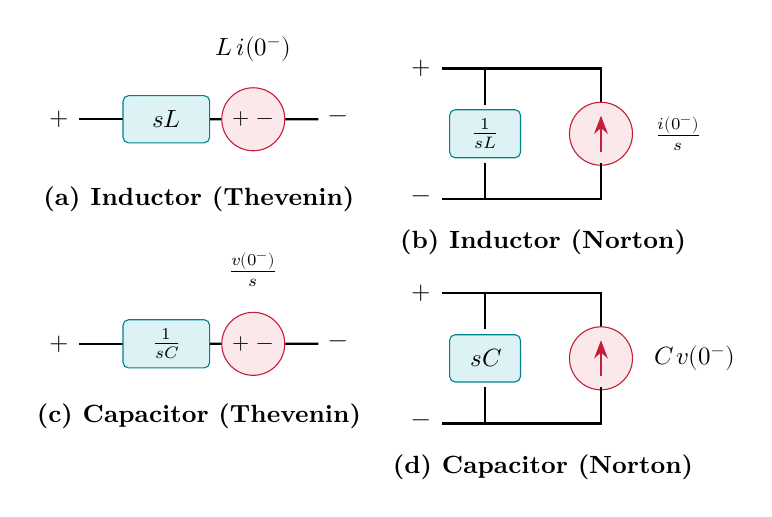
\begin{tikzpicture}[scale=0.92, every node/.style={font=\small}]
  % Inductor Thevenin (Series)
  \draw[thick] (0,2.5) node[left] {$+$} -- (0.6,2.5);
  \node[draw=myteal, fill=hdrteal, minimum width=1.1cm, minimum height=0.6cm, rounded corners=2pt] (ZL) at (1.2,2.5) {$sL$};
  \draw[thick] (ZL.east) -- (2.0,2.5);
  \node[sourcenode, minimum size=0.8cm] (VL) at (2.4,2.5) {};
  \node at (2.4, 2.5) {\footnotesize $+ \,\, -$};
  \node[above=0.2cm of VL] {$L\,i(0^-)$};
  \draw[thick] (VL.east) -- (3.3,2.5) node[right] {$-$};
  \node at (1.65, 1.4) {\textbf{(a) Inductor (Thevenin)}};

  % Inductor Norton (Parallel)
  \draw[thick] (5.0,3.2) node[left] {$+$} -- (5.6,3.2) -- (5.6,2.7);
  \node[draw=myteal, fill=hdrteal, minimum width=0.9cm, minimum height=0.6cm, rounded corners=2pt] (YL) at (5.6,2.3) {$\frac{1}{sL}$};
  \draw[thick] (5.6,1.9) -- (5.6,1.4) -- (5.0,1.4) node[left] {$-$};
  \draw[thick] (5.6,3.2) -- (7.2,3.2) -- (7.2,2.7);
  \node[sourcenode, minimum size=0.8cm] (IL) at (7.2,2.3) {};
  \draw[-Stealth, thick, color=myred] (7.2, 2.05) -- (7.2, 2.55);
  \node[right=0.15cm of IL] {$\frac{i(0^-)}{s}$};
  \draw[thick] (7.2,1.9) -- (7.2,1.4) -- (5.6,1.4);
  \node at (6.4, 0.8) {\textbf{(b) Inductor (Norton)}};

  % Capacitor Thevenin (Series)
  \draw[thick] (0,-0.6) node[left] {$+$} -- (0.6,-0.6);
  \node[draw=myteal, fill=hdrteal, minimum width=1.1cm, minimum height=0.6cm, rounded corners=2pt] (ZC) at (1.2,-0.6) {$\frac{1}{sC}$};
  \draw[thick] (ZC.east) -- (2.0,-0.6);
  \node[sourcenode, minimum size=0.8cm] (VC) at (2.4,-0.6) {};
  \node at (2.4, -0.6) {\footnotesize $+ \,\, -$};
  \node[above=0.2cm of VC] {$\frac{v(0^-)}{s}$};
  \draw[thick] (VC.east) -- (3.3,-0.6) node[right] {$-$};
  \node at (1.65, -1.6) {\textbf{(c) Capacitor (Thevenin)}};

  % Capacitor Norton (Parallel)
  \draw[thick] (5.0,0.1) node[left] {$+$} -- (5.6,0.1) -- (5.6,-0.4);
  \node[draw=myteal, fill=hdrteal, minimum width=0.9cm, minimum height=0.6cm, rounded corners=2pt] (YC) at (5.6,-0.8) {$sC$};
  \draw[thick] (5.6,-1.2) -- (5.6,-1.7) -- (5.0,-1.7) node[left] {$-$};
  \draw[thick] (5.6,0.1) -- (7.2,0.1) -- (7.2,-0.4);
  \node[sourcenode, minimum size=0.8cm] (IC) at (7.2,-0.8) {};
  \draw[-Stealth, thick, color=myred] (7.2, -1.05) -- (7.2, -0.55);
  \node[right=0.15cm of IC] {$C\,v(0^-)$};
  \draw[thick] (7.2,-1.2) -- (7.2,-1.7) -- (5.6,-1.7);
  \node at (6.4, -2.3) {\textbf{(d) Capacitor (Norton)}};
\end{tikzpicture}
\end{center}
\end{tcolorbox}

% ===============================================================================
% SECTION 6: FIRST-ORDER NETWORK TRANSIENTS
% ===============================================================================
\section{Transient Analysis of First-Order Networks (RL and RC)}

First-order circuits contain a single equivalent energy-storage element ($L$ or $C$) and are mathematically governed by linear first-order ordinary differential equations.

\subsection{Series RL Network with DC Step Voltage}

Consider a series connection of resistance $R$ and inductance $L$ excited at $t=0$ by a step voltage $V\,u(t)$ with an initial current $i(0^-) = I_0$.

\begin{tcolorbox}[formulabox, title={\textbf{Mathematical Derivation of RL Response}}]
Applying KVL in the transformed $s$-domain:
\begin{equation}
  \frac{V}{s} = R\,I(s) + sL\,I(s) - L\,I_0 \implies I(s)(R + sL) = \frac{V}{s} + L\,I_0
\end{equation}
Solving for the current transform $I(s)$:
\begin{equation}
  I(s) = \frac{V}{s(sL + R)} + \frac{L\,I_0}{sL + R} = \frac{V/L}{s\left(s + \frac{R}{L}\right)} + \frac{I_0}{s + \frac{R}{L}}
\end{equation}
Decomposing the first term via partial fractions:
\begin{equation}
  \frac{V/L}{s\left(s + \frac{R}{L}\right)} = \frac{V/R}{s} - \frac{V/R}{s + \frac{R}{L}}
\end{equation}
Substituting back and collecting terms:
\begin{equation}
  I(s) = \frac{V/R}{s} - \frac{V/R}{s + \frac{R}{L}} + \frac{I_0}{s + \frac{R}{L}}
\end{equation}
Taking the inverse Laplace transform for $t \ge 0$:
\begin{equation}
  i(t) = \frac{V}{R}\left(1 - e^{-\frac{R}{L}t}\right) + I_0\,e^{-\frac{R}{L}t} = \underbrace{\frac{V}{R}}_{\text{Forced (SS)}} + \underbrace{\left(I_0 - \frac{V}{R}\right)e^{-t/\tau}}_{\text{Natural (Transient)}}
\end{equation}
where $\tau = \frac{L}{R}$ is the inductive time constant (in seconds).
\end{tcolorbox}

\begin{tcolorbox}[defbox, title={\textbf{Decomposition into Zero-Input and Zero-State Responses}}]
\begin{itemize}[leftmargin=*]
  \item \textbf{Zero-Input Response (ZIR):} Response due entirely to initial internal stored energy ($V = 0$):
  \begin{equation}
    i_{\text{ZIR}}(t) = I_0\,e^{-t/\tau}
  \end{equation}
  \item \textbf{Zero-State Response (ZSR):} Response due entirely to external applied excitation with zero initial state ($I_0 = 0$):
  \begin{equation}
    i_{\text{ZSR}}(t) = \frac{V}{R}\left(1 - e^{-t/\tau}\right)
  \end{equation}
  \item \textbf{Principle of Linearity:} Total Response = $\text{ZIR} + \text{ZSR} \equiv \text{Natural} + \text{Forced}$.
\end{itemize}
\end{tcolorbox}

\subsection{Series RC Network with DC Step Voltage}

For a series RC circuit excited by $V\,u(t)$ with initial capacitor voltage $v_C(0^-) = V_0$:
\begin{equation}
  \frac{V}{s} = R\,I(s) + \frac{I(s)}{sC} + \frac{V_0}{s} \implies I(s)\left(R + \frac{1}{sC}\right) = \frac{V - V_0}{s}
\end{equation}
Solving for loop current transform $I(s)$ and capacitor voltage transform $V_C(s)$:
\begin{equation}
  I(s) = \frac{V - V_0}{R\left(s + \frac{1}{RC}\right)} \implies i(t) = \frac{V - V_0}{R}\,e^{-t/\tau} \quad (t \ge 0)
\end{equation}
\begin{equation}
  V_C(s) = \frac{V/RC}{s\left(s + \frac{1}{RC}\right)} + \frac{V_0}{s + \frac{1}{RC}} \implies v_C(t) = V\left(1 - e^{-t/\tau}\right) + V_0\,e^{-t/\tau}
\end{equation}
where $\tau = RC$ is the capacitive time constant.

% ===============================================================================
% SECTION 7: SECOND-ORDER NETWORK TRANSIENTS (SERIES & PARALLEL RLC)
% ===============================================================================
\section{Transient Analysis of Second-Order Networks (RLC)}

Second-order circuits contain two uncoupled energy storage elements ($L$ and $C$) whose transient response is described by a second-order linear differential equation.

\subsection{Series RLC Circuit Formulation}

Applying KVL to a series RLC circuit excited by a DC voltage $V\,u(t)$ with zero initial conditions:
\begin{equation}
  R\,i(t) + L\,\frac{di(t)}{dt} + \frac{1}{C}\int_0^t i(\tau)\,d\tau = V
\end{equation}
Taking the Laplace transform with zero initial conditions:
\begin{equation}
  I(s)\left[R + sL + \frac{1}{sC}\right] = \frac{V}{s} \implies I(s)\left[\frac{s^2 L + s R + \frac{1}{C}}{s}\right] = \frac{V}{s}
\end{equation}
\begin{equation}
  I(s) = \frac{V/L}{s^2 + \frac{R}{L}s + \frac{1}{LC}} = \frac{V/L}{s^2 + 2\alpha s + \omega_0^2}
\end{equation}

\begin{tcolorbox}[formulabox, title={\textbf{Standard Second-Order Characteristic Parameters}}]
\begin{equation}
  s^2 + 2\alpha s + \omega_0^2 = 0 \quad \text{or} \quad s^2 + 2\zeta\omega_0 s + \omega_0^2 = 0
\end{equation}
\begin{itemize}[leftmargin=*]
  \item \textbf{Neper Frequency (Attenuation Factor):} $\alpha = \dfrac{R}{2L}$ (rad/s)
  \item \textbf{Undamped Resonant Frequency:} $\omega_0 = \dfrac{1}{\sqrt{LC}}$ (rad/s)
  \item \textbf{Damping Ratio:} $\zeta = \dfrac{\alpha}{\omega_0} = \dfrac{R}{2}\sqrt{\dfrac{C}{L}}$
\end{itemize}
Roots of the characteristic polynomial:
\begin{equation}
  s_{1,2} = -\alpha \pm \sqrt{\alpha^2 - \omega_0^2} = -\zeta\omega_0 \pm \omega_0\sqrt{\zeta^2 - 1}
\end{equation}
\end{tcolorbox}

\subsection{Classification of Damping Regimes}

The nature of the transient response depends strictly on the discriminant $(\alpha^2 - \omega_0^2)$ or damping ratio $\zeta$:

\begin{tcolorbox}[defbox, title={\textbf{Three Classical Damping Regimes}}]
\begin{enumerate}[leftmargin=*]
  \item \textbf{Overdamped ($\zeta > 1 \iff R > 2\sqrt{L/C} \iff \alpha > \omega_0$):}
  The roots $s_1, s_2$ are real, negative, and unequal.
  \begin{equation}
    i(t) = \frac{V}{2\beta L}\left(e^{-(\alpha - \beta)t} - e^{-(\alpha + \beta)t}\right), \quad \text{where } \beta = \sqrt{\alpha^2 - \omega_0^2}
  \end{equation}
  The current rises to a peak and decays sluggishly to zero without any oscillation.

  \item \textbf{Critically Damped ($\zeta = 1 \iff R = 2\sqrt{L/C} \iff \alpha = \omega_0$):}
  The roots are real, negative, and identical: $s_1 = s_2 = -\alpha$.
  \begin{equation}
    i(t) = \frac{V}{L}\,t\,e^{-\alpha t}
  \end{equation}
  Provides the fastest non-oscillatory return to steady-state equilibrium.

  \item \textbf{Underdamped ($\zeta < 1 \iff R < 2\sqrt{L/C} \iff \alpha < \omega_0$):}
  The roots are a pair of complex conjugates in the left-half $s$-plane:
  \begin{equation}
    s_{1,2} = -\alpha \pm j\omega_d, \quad \text{where } \omega_d = \sqrt{\omega_0^2 - \alpha^2} = \omega_0\sqrt{1 - \zeta^2}
  \end{equation}
  $\omega_d$ is the damped natural frequency. The loop current is an exponentially decaying sinusoidal oscillation:
  \begin{equation}
    i(t) = \frac{V}{\omega_d L}\,e^{-\alpha t}\sin(\omega_d t)
  \end{equation}
  The capacitor voltage exhibits oscillatory overshoot:
  \begin{equation}
    v_C(t) = V\left[1 - \frac{e^{-\alpha t}}{\sqrt{1 - \zeta^2}}\sin(\omega_d t + \phi)\right], \quad \phi = \cos^{-1}(\zeta)
  \end{equation}
\end{enumerate}
\end{tcolorbox}

\begin{tcolorbox}[tikzbox, title={\textbf{TikZ Plot: Comparison of Second-Order Step Responses for Different Damping Ratios}}]
\begin{center}
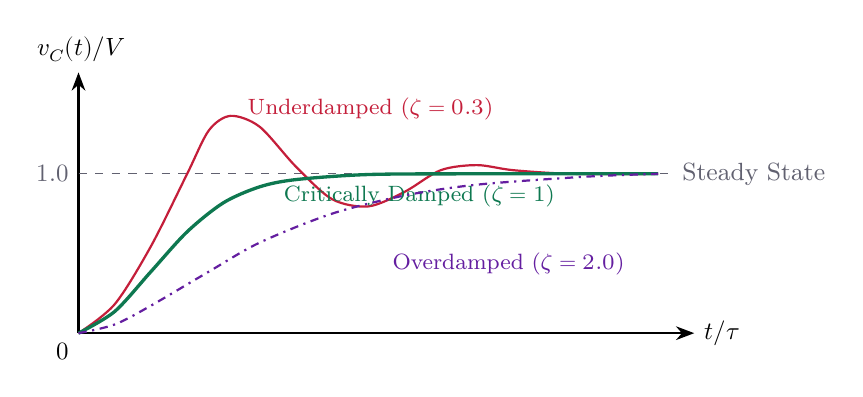
\begin{tikzpicture}[scale=0.92, every node/.style={font=\small}]
  % Axes
  \draw[-Stealth, thick] (0,0) -- (8.5,0) node[right] {$t / \tau$};
  \draw[-Stealth, thick] (0,0) -- (0,3.6) node[above] {$v_C(t) / V$};

  % Steady state line
  \draw[dashed, color=mydark!70] (0,2.2) node[left] {$1.0$} -- (8.2,2.2) node[right] {Steady State};

  % Underdamped Curve (oscillatory overshoot)
  \draw[thick, color=myred, smooth] plot coordinates {
    (0,0) (0.5,0.4) (1.0,1.2) (1.5,2.2) (1.8,2.8) (2.1,3.0) (2.5,2.85) (3.0,2.3)
    (3.5,1.85) (4.0,1.75) (4.5,1.95) (5.0,2.25) (5.5,2.32) (6.0,2.25) (6.8,2.2) (8.0,2.2)
  };
  \node[color=myred, font=\footnotesize, right] at (2.2, 3.1) {Underdamped ($\zeta = 0.3$)};

  % Critically Damped Curve (fastest rise without overshoot)
  \draw[very thick, color=mygreen, smooth] plot coordinates {
    (0,0) (0.5,0.3) (1.0,0.85) (1.5,1.4) (2.0,1.8) (2.5,2.02) (3.0,2.12) (4.0,2.19) (5.5,2.2) (8.0,2.2)
  };
  \node[color=mygreen, font=\footnotesize, above right] at (2.7, 1.6) {Critically Damped ($\zeta = 1$)};

  % Overdamped Curve (sluggish)
  \draw[thick, color=mypurple, dashdotted, smooth] plot coordinates {
    (0,0) (0.5,0.12) (1.0,0.38) (1.8,0.85) (2.5,1.25) (3.5,1.65) (4.5,1.9) (5.5,2.05) (7.0,2.16) (8.0,2.2)
  };
  \node[color=mypurple, font=\footnotesize, below right] at (4.2, 1.25) {Overdamped ($\zeta = 2.0$)};

  % Grid ticks
  \draw (0,0) node[below left] {$0$};
\end{tikzpicture}
\end{center}
\end{tcolorbox}

\subsection{Dual Parallel RLC Network}

In a parallel RLC circuit excited by an independent current step $I\,u(t)$, the dual nodal formulation gives:
\begin{equation}
  \frac{v(t)}{R} + \frac{1}{L}\int_0^t v(\tau)\,d\tau + C\,\frac{dv(t)}{dt} = I
\end{equation}
The characteristic equation and parameters are:
\begin{equation}
  s^2 + \frac{1}{RC}s + \frac{1}{LC} = 0 \implies \alpha = \frac{1}{2RC}, \quad \omega_0 = \frac{1}{\sqrt{LC}}, \quad \zeta = \frac{1}{2R}\sqrt{\frac{L}{C}}
\end{equation}

\newpage
% ===============================================================================
% MANDATORY QUICK REVISION PAGE
% ===============================================================================
\begin{center}
  {\large\bfseries\color{myred} Quick Revision --- Module 3}\\[2pt]
  {\small\color{mydark} Laplace Transforms, Network Transients and Initial Conditions $|$ EC304}
\end{center}
\noindent{\color{myred}\rule{\linewidth}{1.0pt}}
\vspace{2pt}

\begin{tcolorbox}[formulabox, top=5pt, bottom=5pt, title={\textbf{Key Formulas and Network Relations at a Glance}}]
\renewcommand{\arraystretch}{1.20}
\begin{tabularx}{\linewidth}{B{5.0cm} X}
Unilateral Laplace Transform & $F(s) = \int_{0^-}^\infty f(t)\,e^{-st}\,dt, \quad s = \sigma + j\omega$ \\[2pt]
Time Derivative Transform & $\mathcal{L}\{f'(t)\} = sF(s) - f(0^-), \quad \mathcal{L}\{f''(t)\} = s^2F(s) - s f(0^-) - f'(0^-)$ \\[2pt]
Time Shifting Property & $\mathcal{L}\{f(t - t_0)u(t - t_0)\} = e^{-s t_0} F(s) \quad (t_0 \ge 0)$ \\[2pt]
Final Value Theorem & $\lim_{t \to \infty} f(t) = \lim_{s \to 0} s F(s) \quad (\text{poles in open LHP})$ \\[2pt]
Inductor $s$-Domain Model & $V_L(s) = sL I_L(s) - L i_L(0^-) \iff I_L(s) = \frac{V_L(s)}{sL} + \frac{i_L(0^-)}{s}$ \\[2pt]
Capacitor $s$-Domain Model & $V_C(s) = \frac{I_C(s)}{sC} + \frac{v_C(0^-)}{s} \iff I_C(s) = sC V_C(s) - C v_C(0^-)$ \\[2pt]
First-Order Step Response & $x(t) = x(\infty) + [x(0^+) - x(\infty)]e^{-t/\tau}, \quad \tau_{RL} = \frac{L}{R}, \; \tau_{RC} = RC$ \\[2pt]
Series RLC Damping Parameters & $\alpha = \frac{R}{2L}, \quad \omega_0 = \frac{1}{\sqrt{LC}}, \quad \zeta = \frac{\alpha}{\omega_0} = \frac{R}{2}\sqrt{\frac{C}{L}}$ \\[2pt]
Damped Frequency & $\omega_d = \sqrt{\omega_0^2 - \alpha^2} = \omega_0\sqrt{1 - \zeta^2} \quad (\text{for } \zeta < 1)$ \\[2pt]
\end{tabularx}
\end{tcolorbox}

\begin{tcolorbox}[defbox, top=5pt, bottom=5pt, title={\textbf{One-Line Definitions}}]
\begin{itemize}[leftmargin=*, itemsep=1.0pt, topsep=0pt]
  \item \textbf{Singularity Function:} A function exhibiting discontinuities in its value or its higher-order time derivatives.
  \item \textbf{Unit Impulse $\delta(t)$:} A generalized function of infinite height, zero width, and unit integral area at $t=0$.
  \item \textbf{Lower Limit $0^-$:} The instant immediately prior to switching, capturing jump discontinuities and initial states.
  \item \textbf{Zero-Input Response (ZIR):} System response produced solely by initial stored energy with external sources zeroed.
  \item \textbf{Zero-State Response (ZSR):} System response produced solely by applied excitations with zero initial stored energy.
  \item \textbf{Time Constant ($\tau$):} Time required for a first-order transient response to decay to $36.8\%$ ($1/e$) of initial value.
  \item \textbf{Neper Frequency ($\alpha$):} Exponential damping attenuation factor governing the rate of response decay.
  \item \textbf{Undamped Resonant Frequency ($\omega_0$):} Natural oscillation frequency of an LC circuit in the absence of resistance.
  \item \textbf{Damping Ratio ($\zeta$):} Dimensionless ratio $\alpha/\omega_0$ determining whether a second-order circuit oscillates.
  \item \textbf{Critically Damped Circuit:} Second-order circuit with $\zeta=1$ returning to steady state in minimum non-oscillatory time.
\end{itemize}
\end{tcolorbox}

\begin{tcolorbox}[exambox, title={\textbf{Frequently Asked / Viva Questions}}]
\begin{enumerate}[topsep=0pt, label=\textbf{Q\arabic*.}, itemsep=4pt]
  \item \Q{Why cannot inductor current change instantaneously in a finite circuit?}
  Stored magnetic energy is $W = \frac{1}{2}L i_L^2$. An instantaneous change requires infinite power ($P = \frac{dW}{dt} \to \infty$) and infinite voltage ($v_L = L \frac{di}{dt} \to \infty$), which is impossible with finite sources. Hence, $i_L(0^+) = i_L(0^-)$.

  \item \Q{Why does an uncharged capacitor act as a short circuit at $t = 0^+$?}
  Since $v_C(0^+) = v_C(0^-) = 0\text{ V}$, the terminal voltage is zero immediately after switching while current flows freely. An element supporting finite current with zero voltage drop behaves identically to an ideal short circuit.

  \item \Q{Explain the physical necessity of the lower limit $0^-$ in unilateral Laplace transforms.}
  The $0^-$ limit captures Dirac delta impulses $\delta(t)$ acting at $t=0$ and accounts for pre-switching initial conditions ($i_L(0^-), v_C(0^-)$). A lower limit of $0^+$ would omit impulses occurring at the switching origin.

  \item \Q{State the validity condition for applying the Final Value Theorem.}
  $\lim_{t \to \infty} f(t) = \lim_{s \to 0} sF(s)$ is valid strictly if all poles of $sF(s)$ lie in the open left-half $s$-plane. If poles lie on the imaginary axis (e.g. sustained sinusoids) or in the right-half plane, FVT produces incorrect results.

  \item \Q{Distinguish between natural and forced responses in circuit transients.}
  The natural (transient) response depends solely on circuit storage elements ($R, L, C$) and decays to zero. The forced (steady-state) response is sustained by external driving sources and mirrors their functional form.

  \item \Q{Under what switching condition is an AC RL circuit completely transient-free?}
  In an RL circuit excited by $v(t) = V_m\sin(\omega t + \theta)$, transient-free operation occurs when switching at $\theta - \phi = 0$ or $\pi$ (where $\phi = \tan^{-1}\frac{\omega L}{R}$), matching prospective steady-state current to the initial zero current.

  \item \Q{How does the Norton $s$-domain model of an inductor differ from its Thevenin form?}
  The Thevenin form consists of an impedance $sL$ in series with an opposing voltage source $L i_L(0^-)$. The Norton form comprises an admittance $\frac{1}{sL}$ in parallel with a current source $\frac{i_L(0^-)}{s}$ pointing in the direction of $i_L$.

  \item \Q{Define damping ratio $\zeta$ and give its formulas for series and parallel RLC circuits.}
  $\zeta = \alpha / \omega_0$. For series RLC: $\zeta = \frac{R}{2}\sqrt{\frac{C}{L}}$. For parallel RLC: $\zeta = \frac{1}{2R}\sqrt{\frac{L}{C}}$.

  \item \Q{Why is critical damping ($\zeta = 1$) preferred in analog meters and galvanometers?}
  Critical damping ensures the pointer reaches its steady deflection in the shortest possible time without oscillatory overshoot or sluggish delay, enabling fast, accurate readings.

  \item \Q{What is the circuit significance of the unit doublet $\delta'(t)$?}
  The unit doublet represents $\frac{d\delta}{dt}$. In circuits, it arises from impulsive current injection across inductors or impulse voltage across capacitors, abruptly altering state variables at $t=0$.
\end{enumerate}
\end{tcolorbox}

\begin{tcolorbox}[tikzbox, title={\textbf{Summary Matrix: Comprehensive Comparison of First- and Second-Order Transients}}]
\par\vspace{3pt}\noindent
\begingroup
\setlength{\tabcolsep}{4.5pt}
\setlength{\extrarowheight}{2.5pt}
\renewcommand{\arraystretch}{1.30}
\begin{tabularx}{\linewidth}{|B{2.8cm}|B{3.2cm}|B{3.2cm}|Y|}
\hline
\multicolumn{1}{|c|}{\textbf{Circuit Type}} & \multicolumn{1}{c|}{\textbf{Time Const. / Damping}} & \multicolumn{1}{c|}{\textbf{Characteristic Roots}} & \multicolumn{1}{c|}{\textbf{Transient Response Characteristic}} \\
\hline
Series RL & $\tau = \dfrac{L}{R}$ & $s = -\dfrac{R}{L}$ & Monotonic exponential rise or decay; no oscillation. \\
\hline
Series RC & $\tau = RC$ & $s = -\dfrac{1}{RC}$ & Monotonic exponential voltage change; current jump at $t=0^+$. \\
\hline
Series RLC Overdamped & $\alpha = \dfrac{R}{2L} > \omega_0, \; \zeta > 1$ & $s_{1,2} = -\alpha \pm \sqrt{\alpha^2 - \omega_0^2}$ & Sum of two decaying exponentials; sluggish, non-oscillatory. \\
\hline
Series RLC Critically Damped & $\alpha = \omega_0, \; \zeta = 1$ & $s_1 = s_2 = -\alpha$ & Rapid monotonic return to equilibrium without overshoot ($(A_1+A_2 t)e^{-\alpha t}$). \\
\hline
Series RLC Underdamped & $\alpha < \omega_0, \; \zeta < 1$ & $s_{1,2} = -\alpha \pm j\omega_d$ & Damped sinusoidal oscillations with decaying envelope $e^{-\alpha t}$. \\
\hline
Parallel RLC & $\alpha = \dfrac{1}{2RC}, \; \zeta = \dfrac{1}{2R}\sqrt{\dfrac{L}{C}}$ & $s_{1,2} = -\alpha \pm \sqrt{\alpha^2 - \omega_0^2}$ & Dual of series RLC; higher $R$ produces lower damping (oscillatory). \\
\hline
\end{tabularx}
\endgroup
\end{tcolorbox}

\end{document}
